\chapter{Results}
\label{ch:results}



\section{Evaluation setup}

\subsection{Comparison Targets}
\label{sec:comparison_targets}
To evaluate the performance of the \gls{rtic} port to RISC-V, there are two natural options. Either the performance of the OS is compared to another OS that is running on RISC-V. In this case, this would be FreeRTOS, since it is widely used in the group. With this method, one could identify advantages or disadvantages of \gls{rtic}.

The other option is to compare the port of the OS to its original version on its native platform. In this case, this would be \gls{rtic} on ARM Cortex-M. This makes it possible to identify performance differences between the two architectures. Since this is more interesting for the group, that mainly works in hardware and not OS development.

To compare two RTOSs there are again two natural options. One could write a program with a realistic workload, and run it on both setups that should be compared. To identify differences in hardware performance, it makes more sense to compare the core transitions of the ROTS on both platforms. With this setup, we can clearly identify where our RISC-V implementation has room for improvement compared to ARM.

\subsection{Platform}
The platforms that are used to perform the measurements were on one side a physical NUCLEO-F103RB evaluation board with a built-in STM32F103RB processor.

On the other side, we use an RTL simulation of the controlPULP IP. 

\subsection{Time Measurement}
To measure the time that certain operations take, there are a few options. If an RTL simulation is used, the exact points in time at which an instruction is executed can directly be read out.

Another possibility would be to toggle GPIO pins at certain points in time, and measure the time in between with an oscilloscope. This however only works on a physical device and introduces a lot of measurement uncertainty.

In any other setup, however, it comes down to counting cycles. These can either be counted using a timer that is attached to the main clock. In this case, the timer value can simply be read out. Or it can be counted by reading out the processor's cycle count registers. 

Since counting cycles is the only option that is available on both platforms, it is the best way to acquire measurements that are actually comparable. Therefore, we use the built-in cycle counters for time measurements. On RISC-V they are even a bit more accurate than timer value readouts, since the timer value read needs to load the address of the timer value register into a temporary register, while the cycle counter can be accessed with one single \gls{csr} read.

\section{Core Transitions}
\label{sec:core_transitions}

We decided to measure core OS transitions for the reasons explained in section \ref{sec:comparison_targets}. In the following, all core transitions that are measured are described. We mainly focus on task spawns, since they are the most important actions in \gls{rtic}. To get an understanding of how the task spawning works in \gls{rtic}, refer to section \ref{sec:task_dispatcher}.

\subsection{Hardware Task Spawn}

The simplest transition to measure is the spawn time of a hardware tasks. In \gls{rtic}, hardware tasks, are interrupt handlers that are bound to an external interrupt. In our setup, we pended the external interrupt in software, and measured the cycles from before the pending statement to the first instruction of the interrupt handler function. This means after the context switch and interrupt handler function prologue.

\subsection{Task Spawn Higher Priority}

\begin{figure}
  \centerfloat
  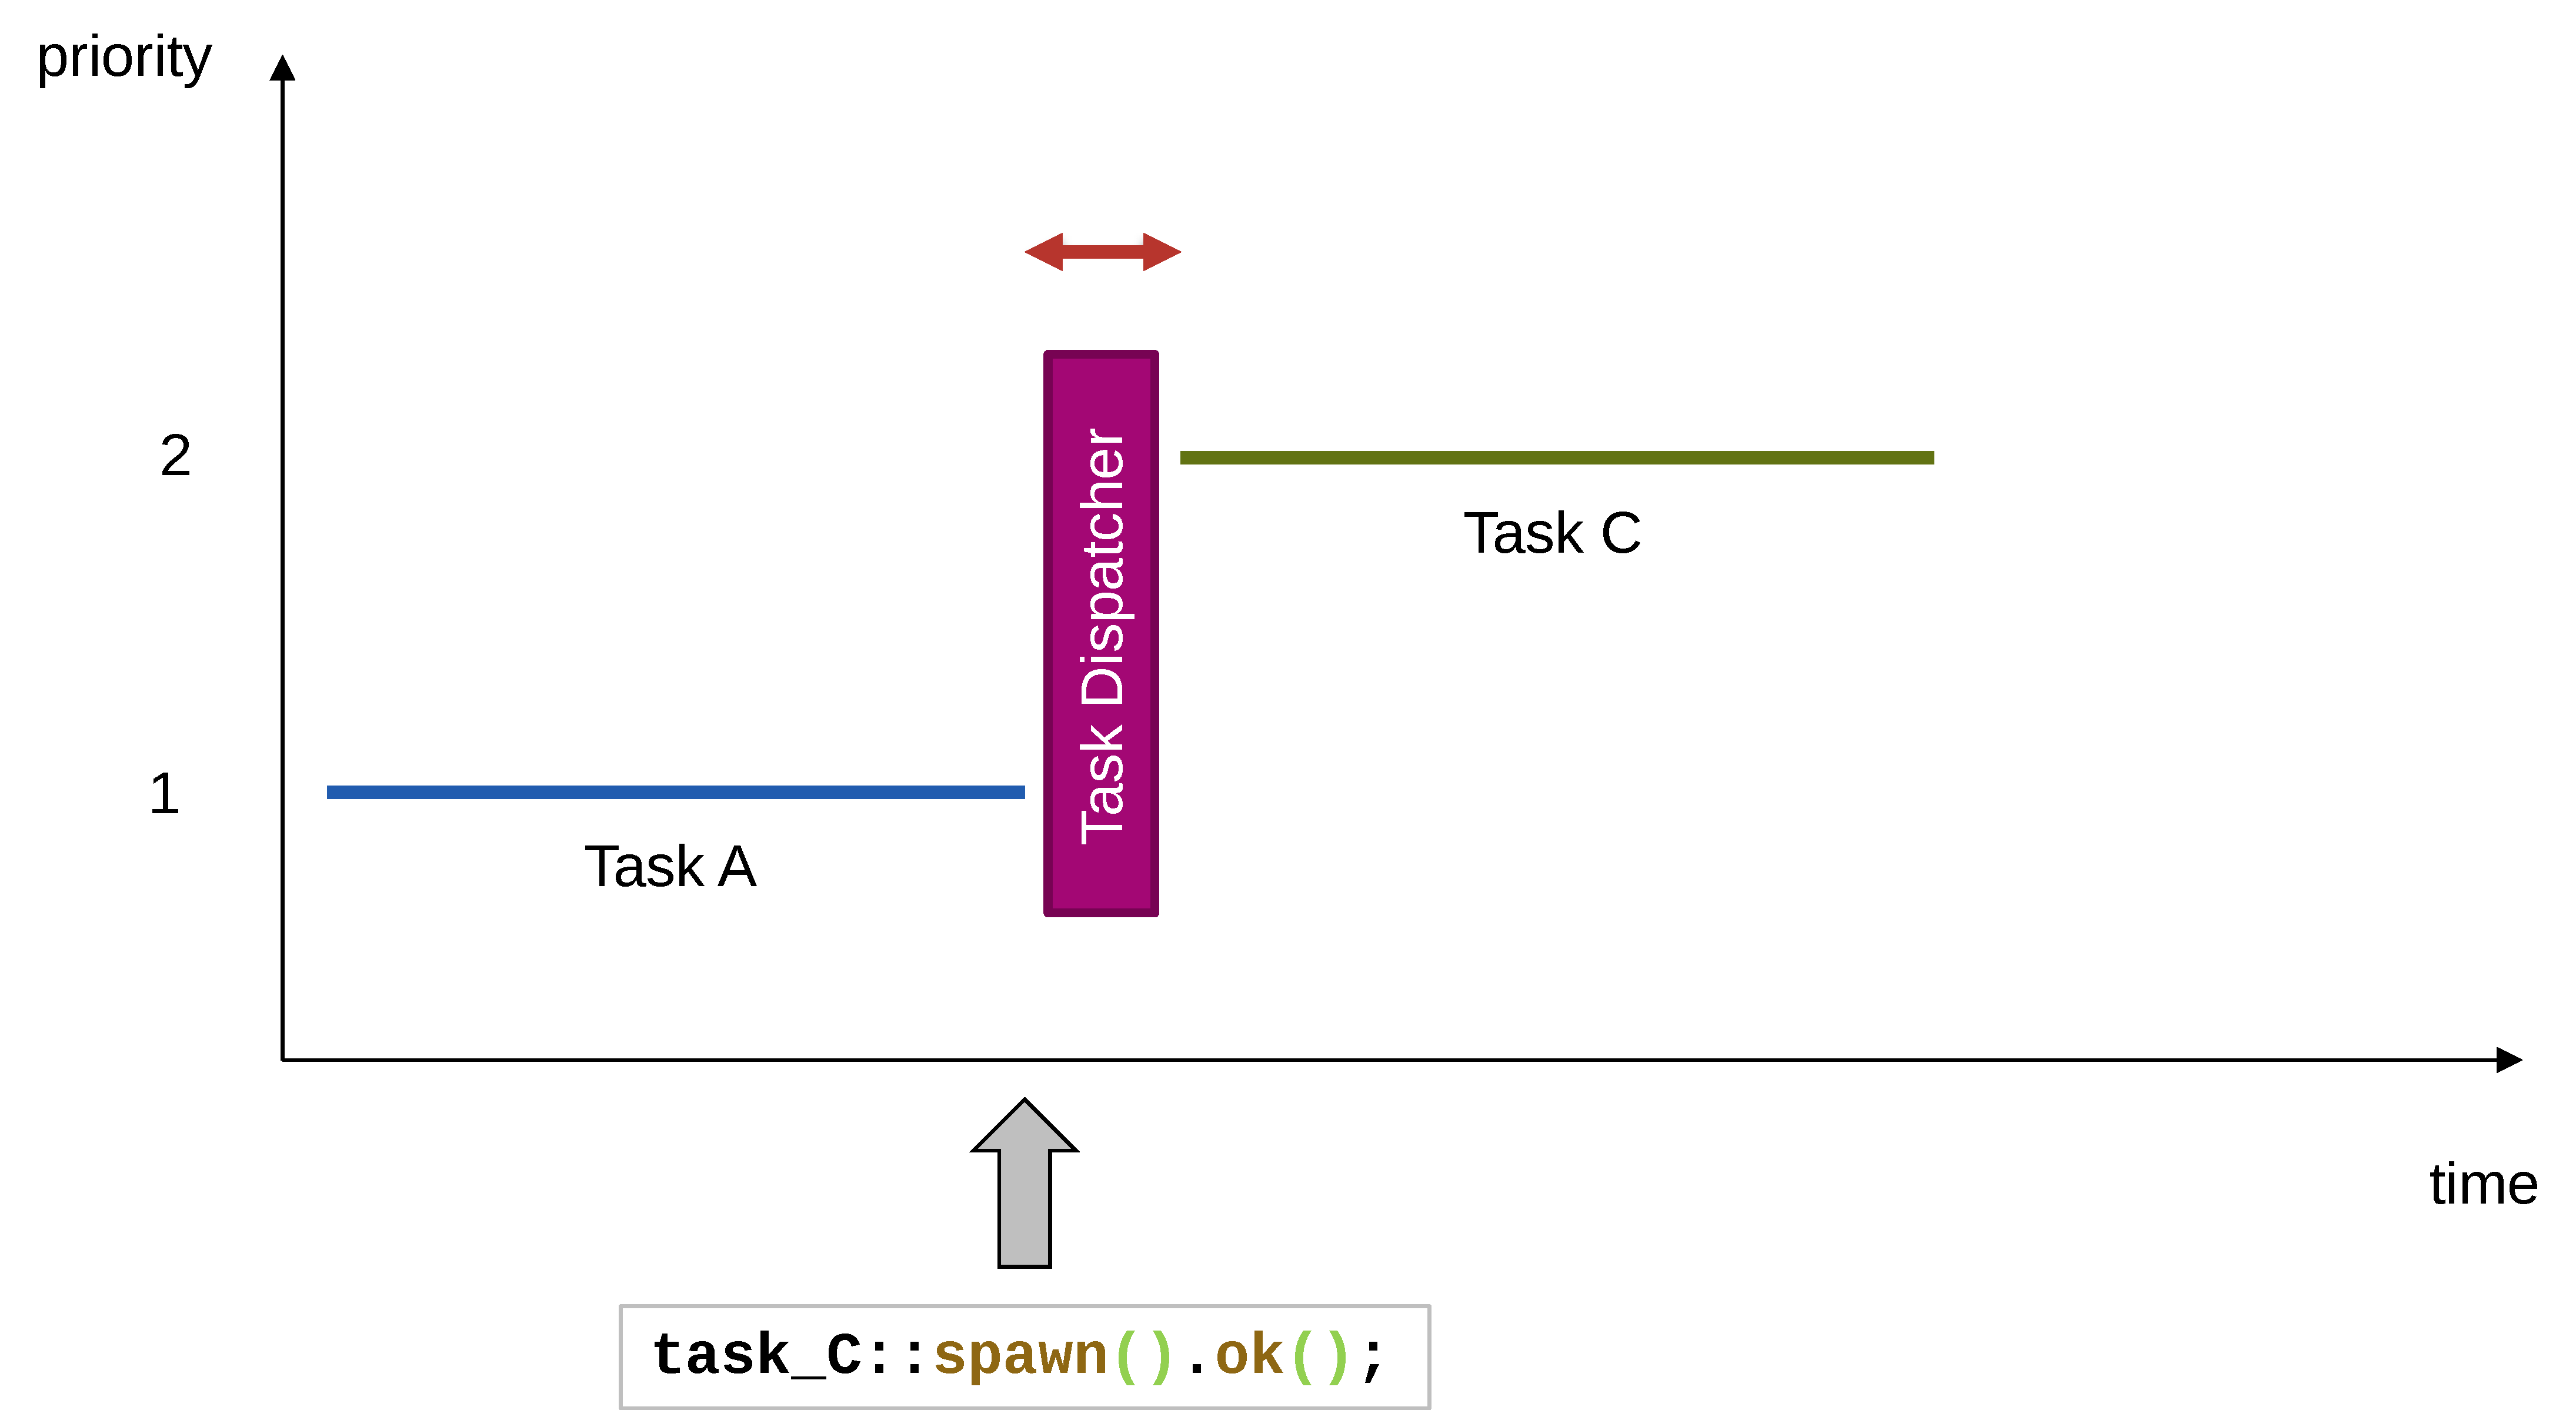
\includegraphics[width=\textwidth]{fig/spawn_prio_high.svg.pdf}
  % Note: We do not have the SVG source file for the image above, so we have to put the PDF under version control.
  \caption{Spawn Task with Higher Priority}%
  \label{fig:spawn_prio_high}
  % Note: The `\label{}` can be on the line after the `\caption{}` if the `\caption{}` line ends with a comment.
\end{figure}

If a task of higher priority (task C) is spawned, the original task is preempted immediately. See figure~\ref{fig:spawn_prio_high}.
We measured the cycles from directly before the execution of the \texttt{task_C::spawn().ok()} statement until the first instruction of the task C Rust function.
This includes the enqueuing of the task into the ready queue of the task dispatcher, the pending of the interrupt associated with the task dispatcher for priority 2, the context switch to the new interrupt handler, the dequeuing of task C, and finally, the prologue of the Rust function of task C.

\subsection{Task Spawn Lower Priority}

\begin{figure}
  \centerfloat
  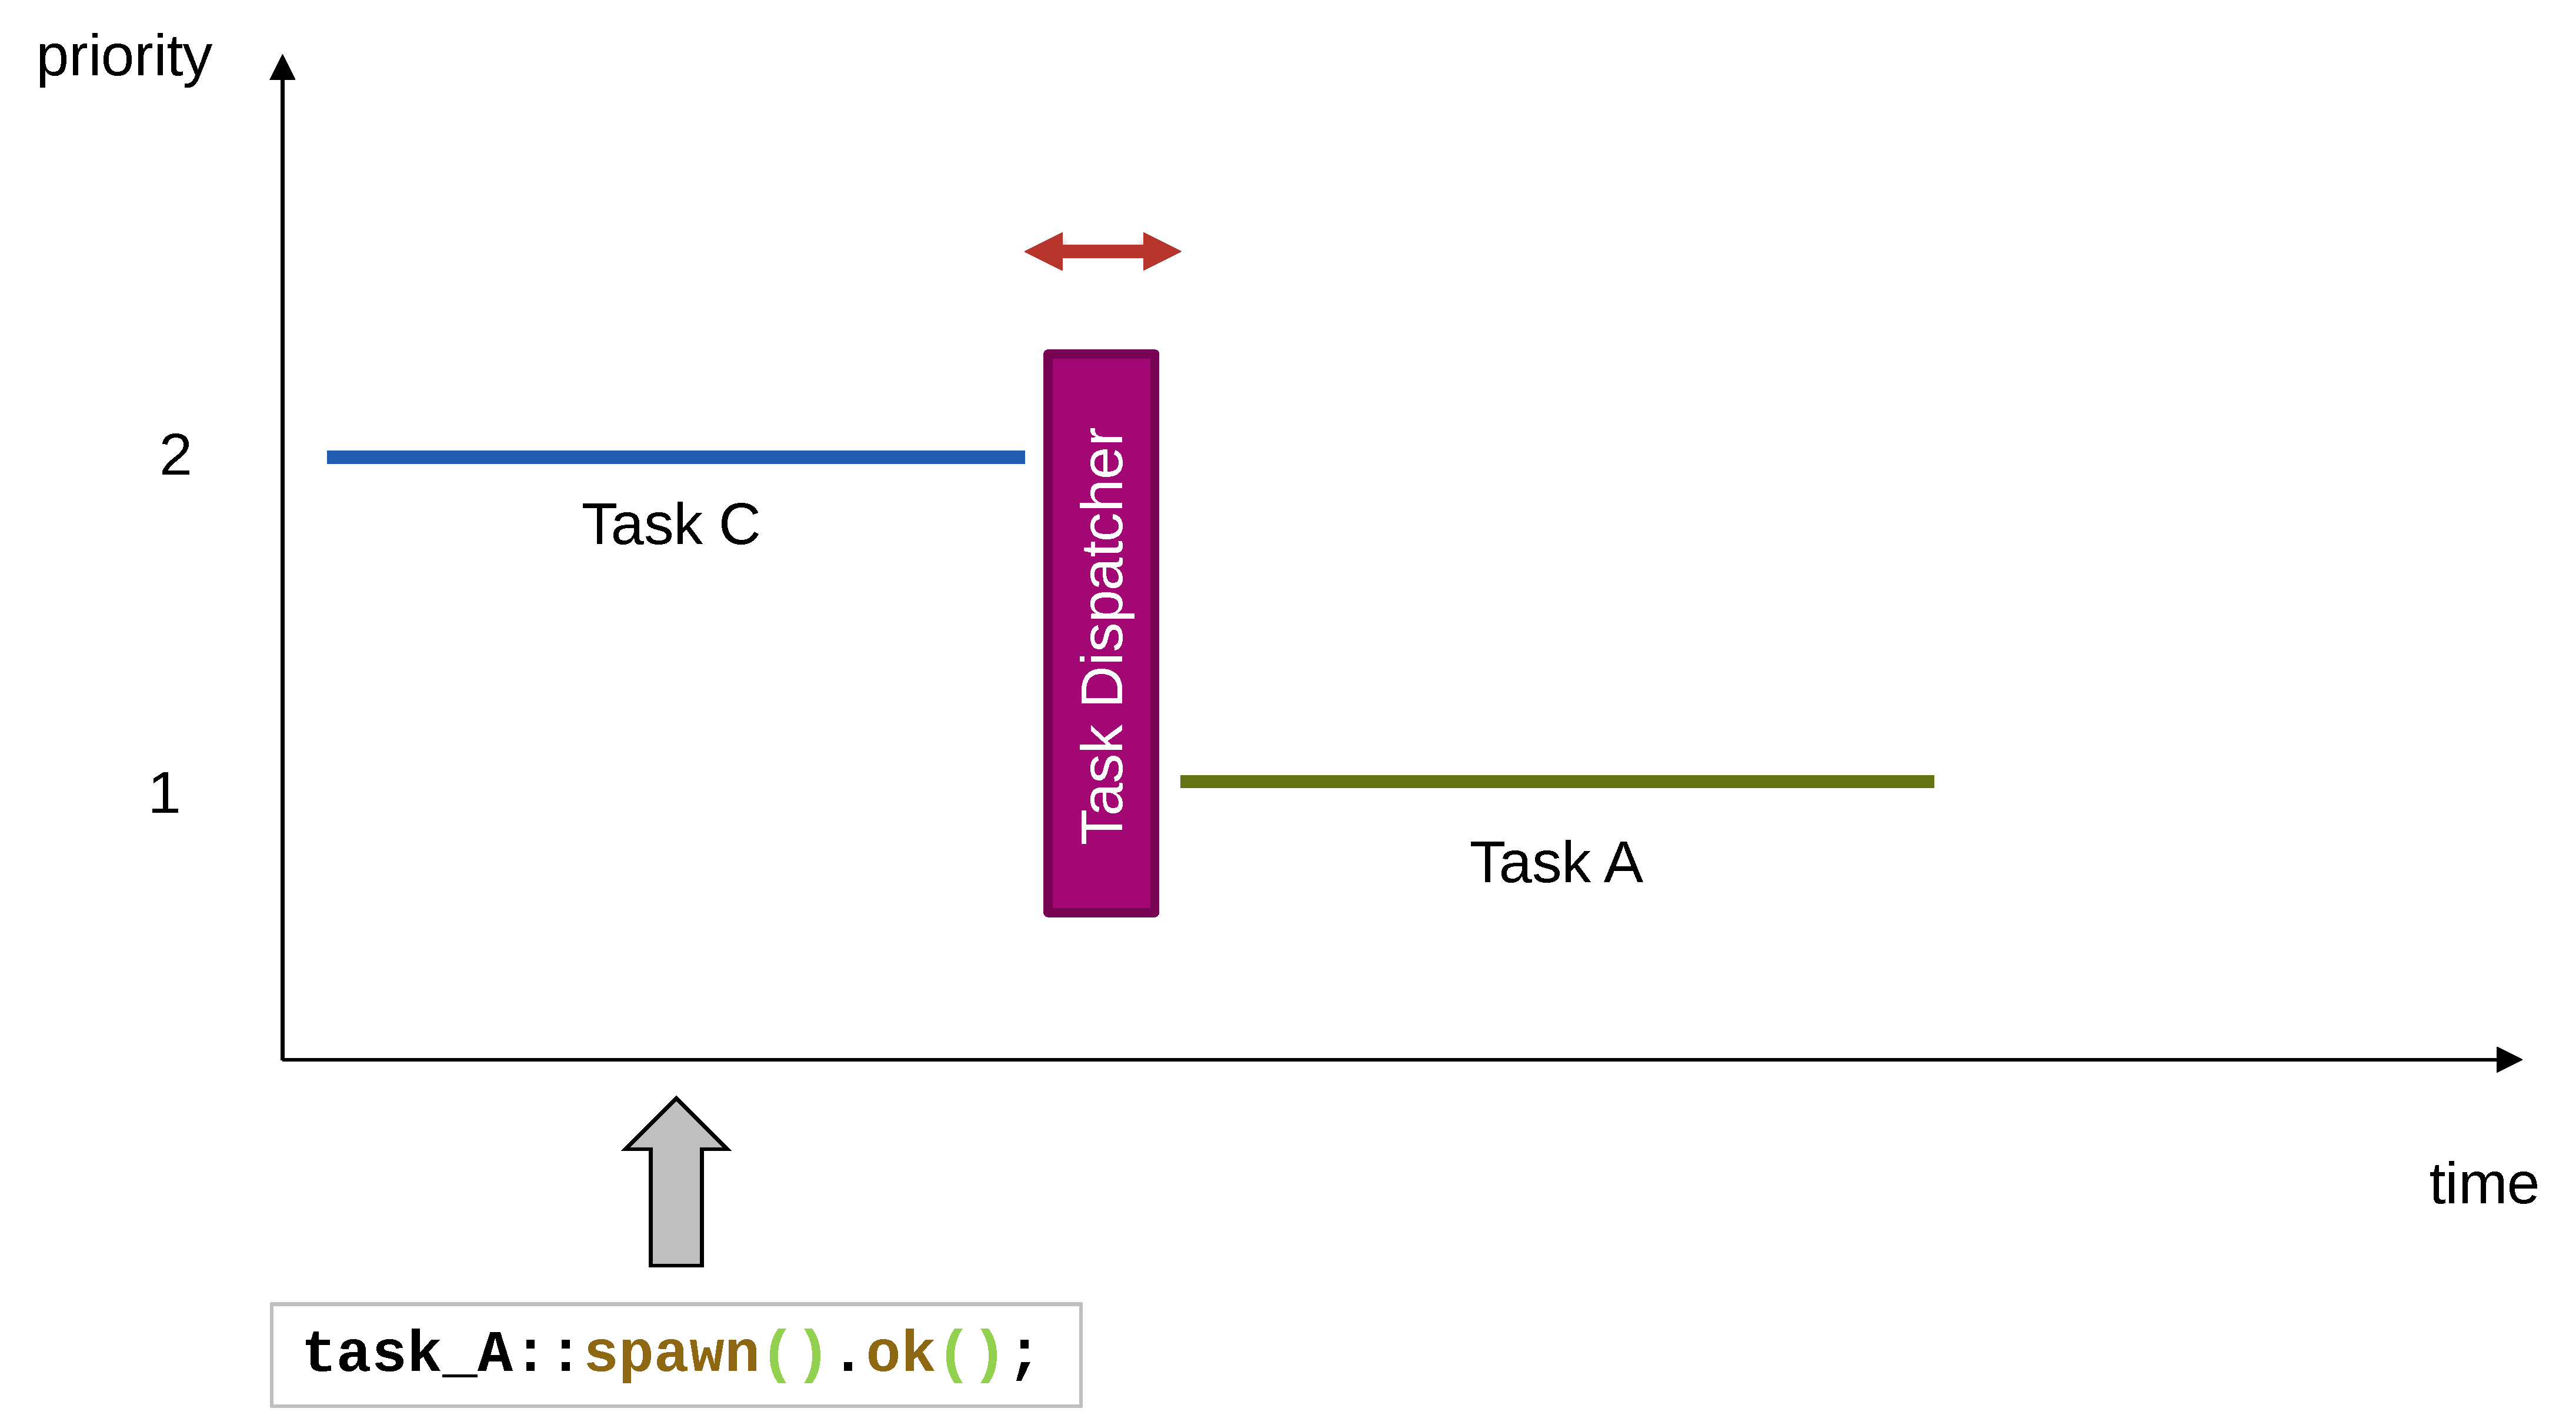
\includegraphics[width=\textwidth]{fig/spawn_prio_low.svg.pdf}
  % Note: We do not have the SVG source file for the image above, so we have to put the PDF under version control.
  \caption{Spawn Task with Lower Priority}%
  \label{fig:spawn_prio_low}
  % Note: The `\label{}` can be on the line after the `\caption{}` if the `\caption{}` line ends with a comment.
\end{figure}

If a task of lower priority is spawned (task A), the new task is enqueued into the ready queue of its task dispatcher, and the corresponding interrupt is pended in software. But since it has lower priority, it does not fire immediately, and the original task (task C) will finish execution first.
In this transition, we measure the cycles between the last instruction of the Rust function of task C and the first instruction of the Rust function of task A. See figure~\ref{fig:spawn_prio_low}.
This includes the epilogue of task C, the interrupt context switch, the dequeuing of task A and the prologue of task A.

\subsection{Task Spawn Equal Priority}

\begin{figure}
  \centerfloat
  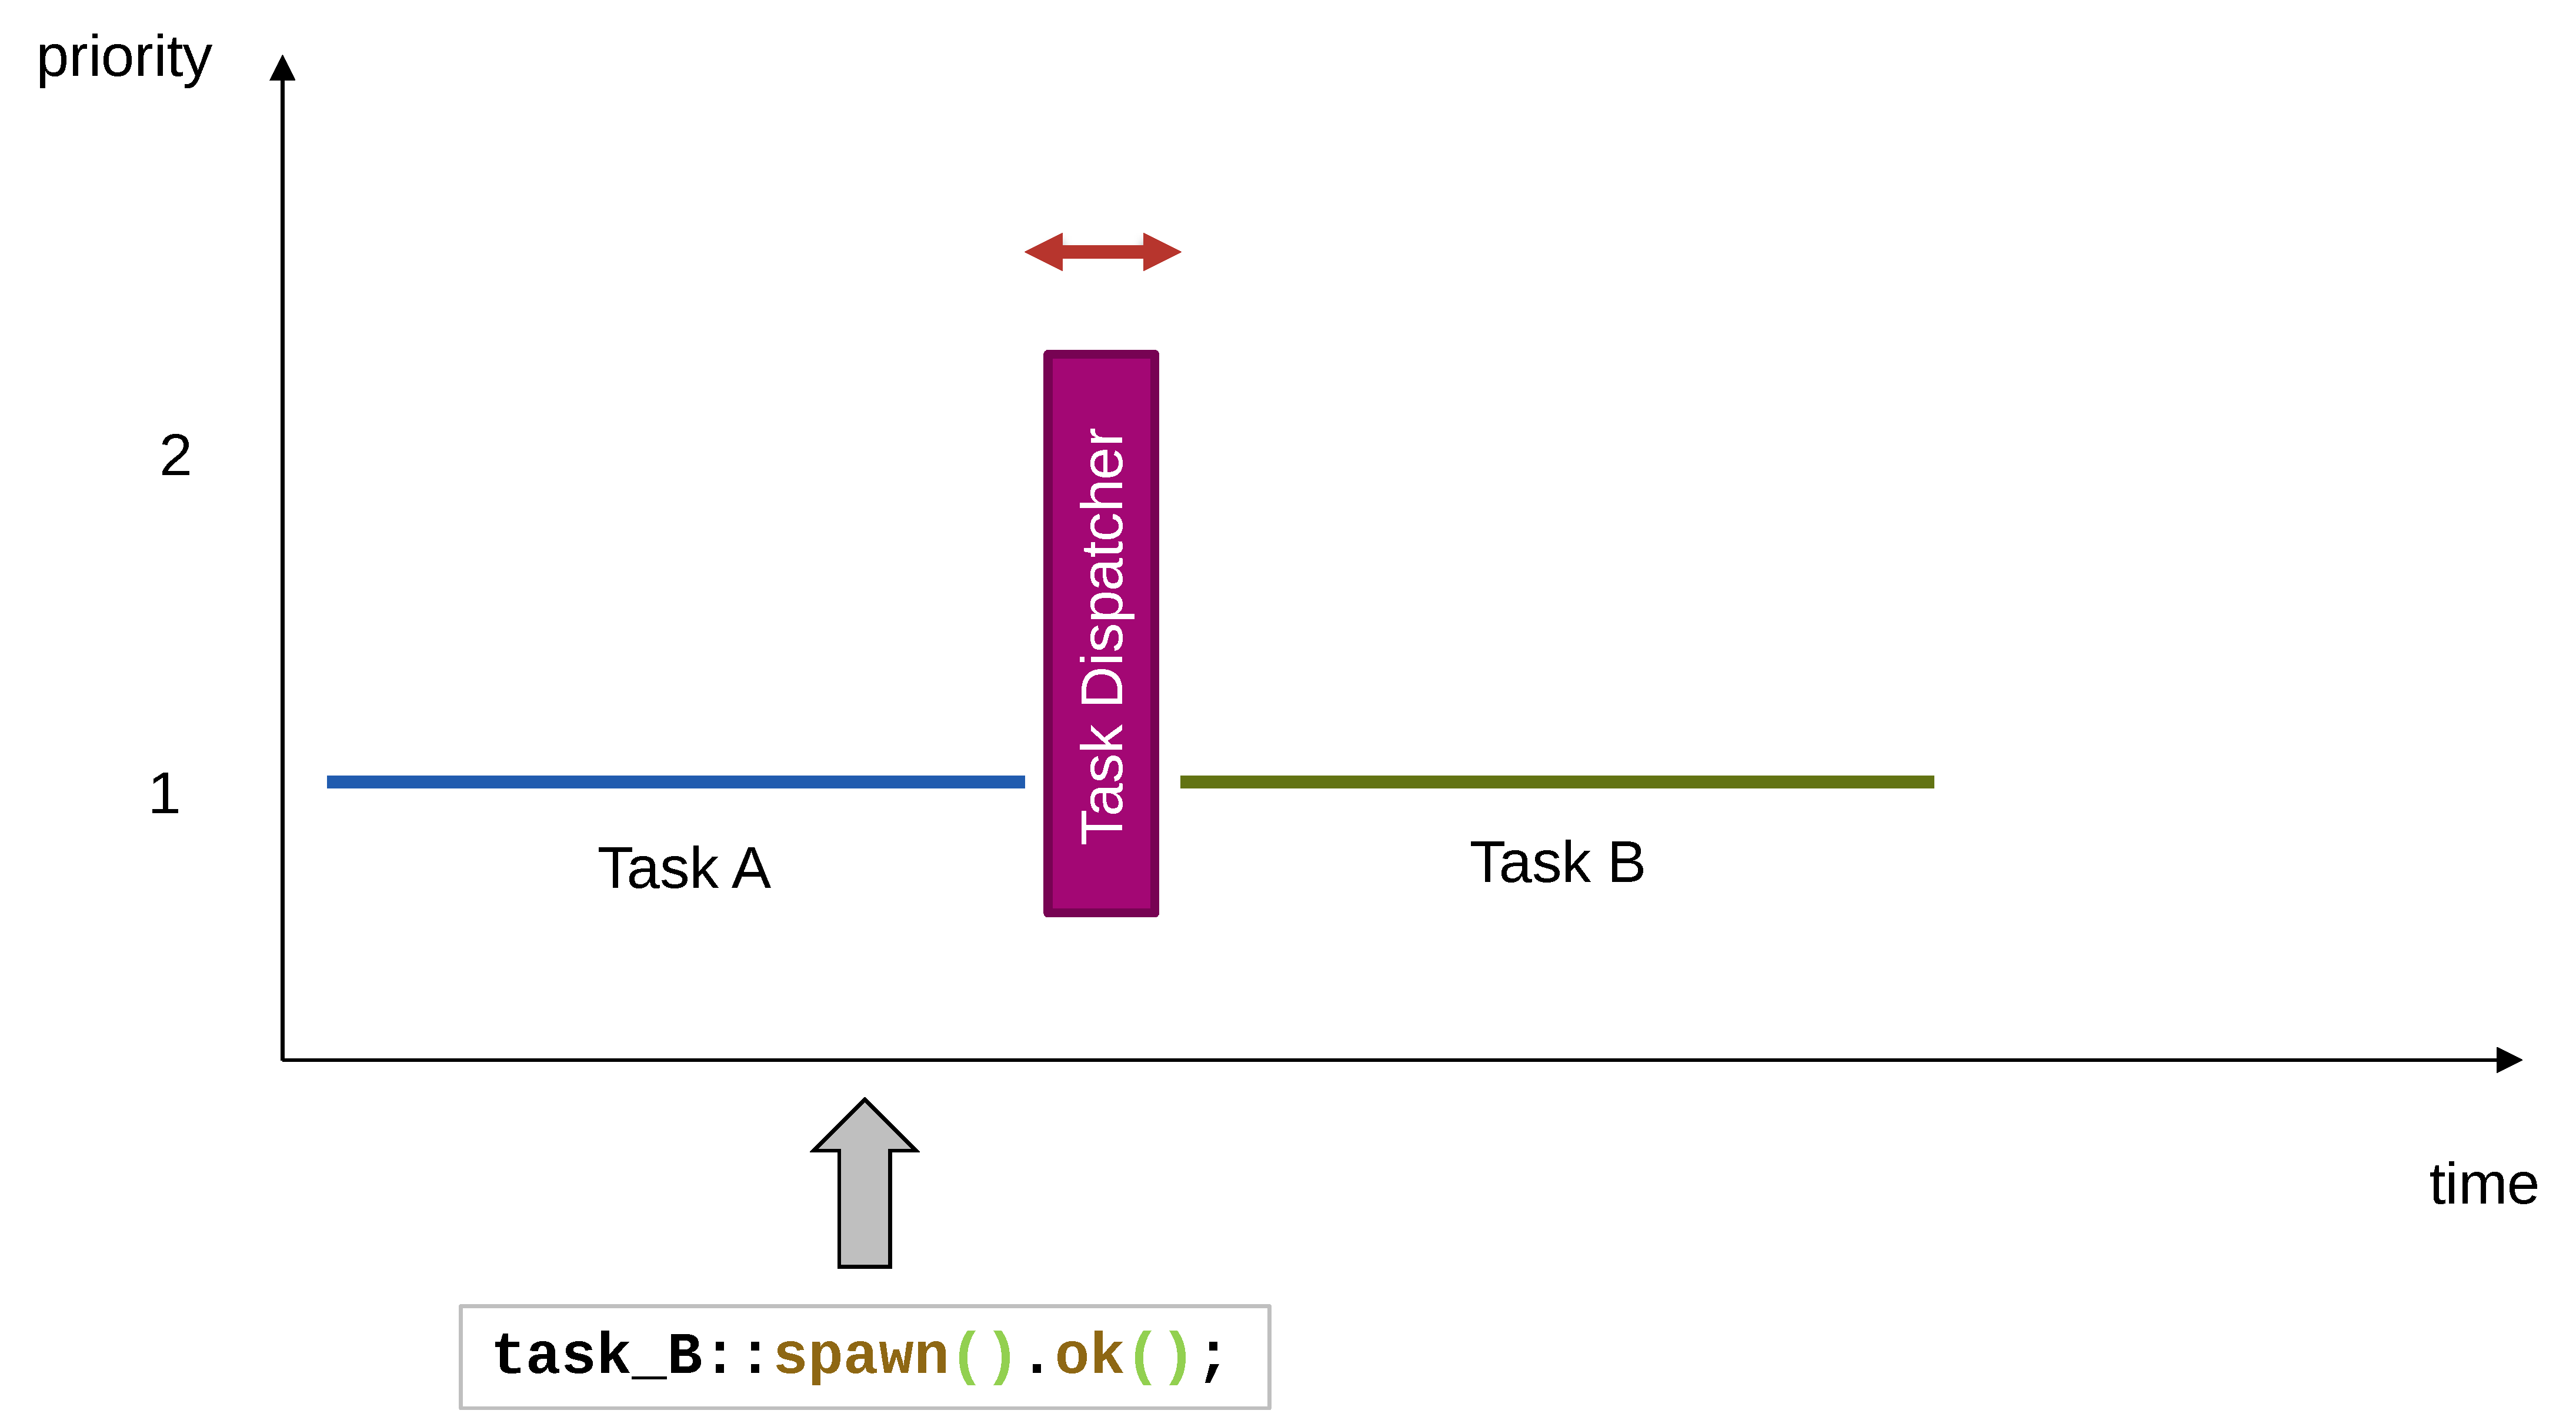
\includegraphics[width=\textwidth]{fig/spawn_prio_equal.svg.pdf}
  % Note: We do not have the SVG source file for the image above, so we have to put the PDF under version control.
  \caption{Spawn Task with Equal Priority}%
  \label{fig:spawn_prio_equal}
  % Note: The `\label{}` can be on the line after the `\caption{}` if the `\caption{}` line ends with a comment.
\end{figure}

If a task of equal priority (task B) is spawned, the new task is enqueued into the ready queue of its task dispatcher, and the corresponding interrupt is pended in software. However, the pended interrupt is actually the same that is currently executing, since there is only one task dispatcher per priority. This means, that the current task (task A) will run until completion. Then the task dispatcher that is already running will dequeue the new task and run it directly. So no context switch is necessary. Therefore, we measure the number of cycles between the last instruction of task A and the first instruction of task B. See figure~\ref{fig:spawn_prio_equal}.

This includes the epilogue of task A, the dequeuing of task B and the prologue of task B.

\subsection{Timed Task Spawn}

\begin{figure}
  \centerfloat
  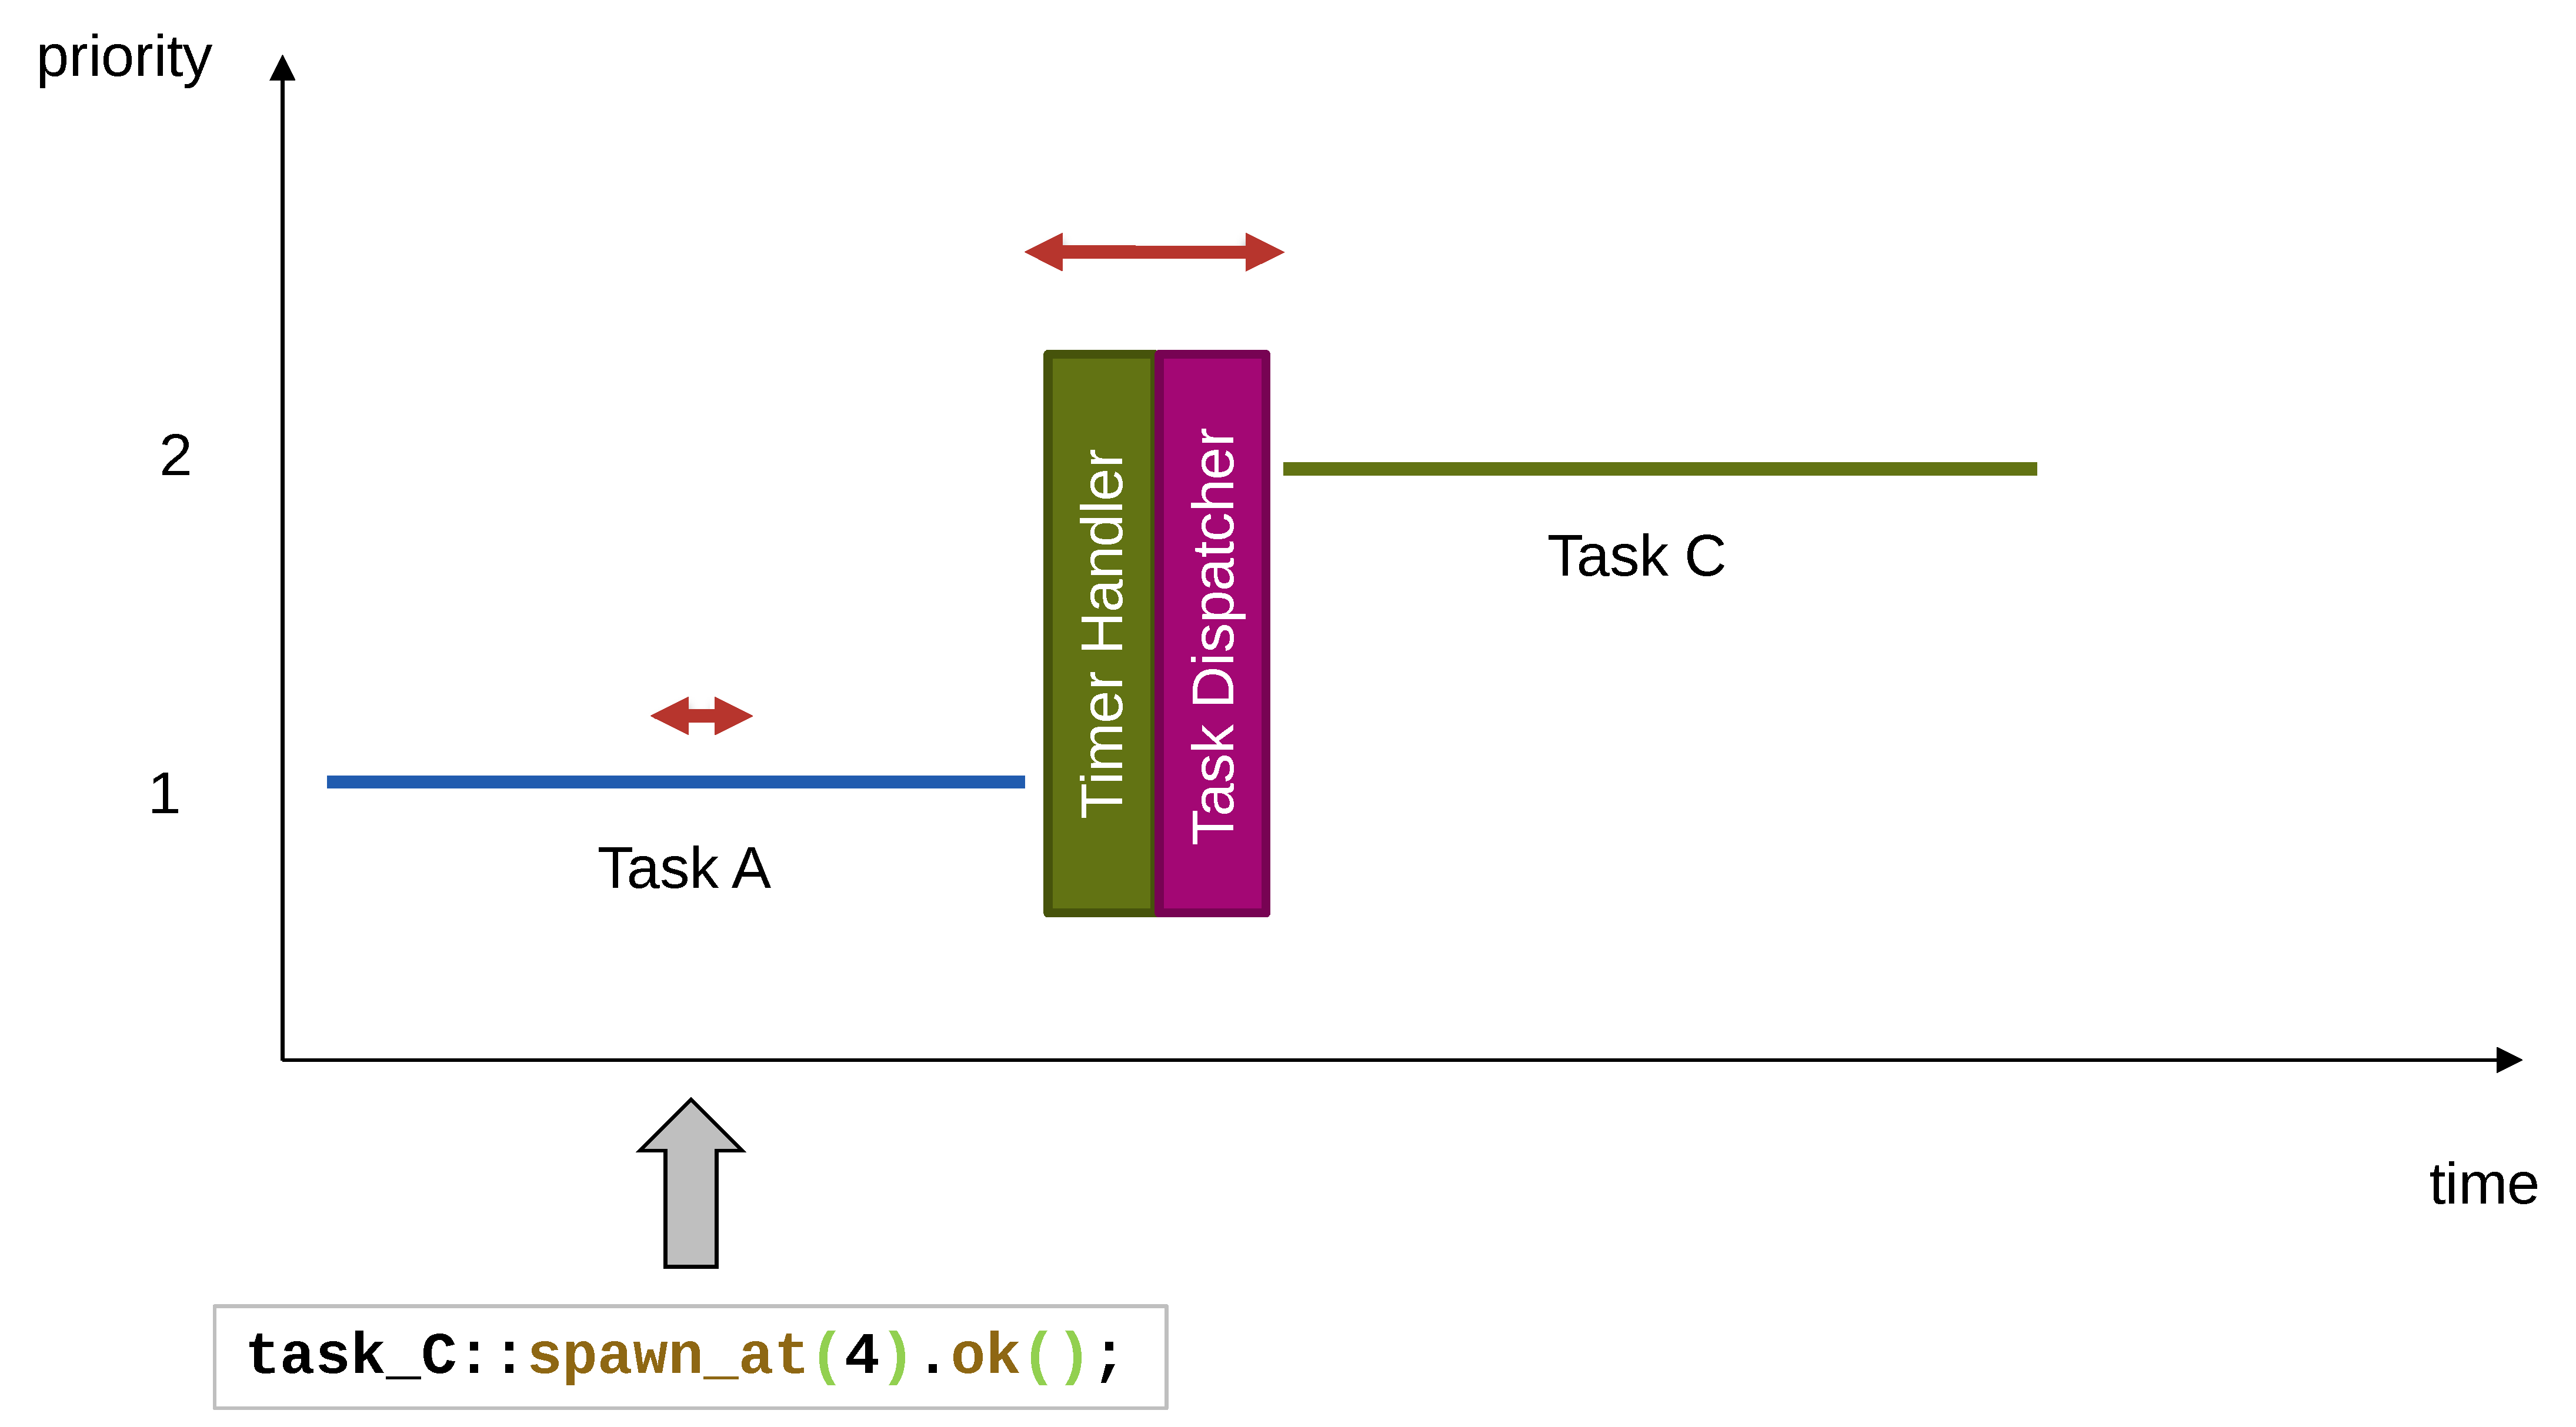
\includegraphics[width=\textwidth]{fig/spawn_prio_timed.svg.pdf}
  % Note: We do not have the SVG source file for the image above, so we have to put the PDF under version control.
  \caption{Spawning of a Timed Task}%
  \label{fig:spawn_prio_timed}
  % Note: The `\label{}` can be on the line after the `\caption{}` if the `\caption{}` line ends with a comment.
\end{figure}

In the spawning process of a timed task (task C), there are two interesting sequences to measure. First, the scheduling of task C. And secondly, the effective start time of task C. See figure~\ref{fig:spawn_prio_timed}.

For the scheduling, the task first is sorted into the timer queue. Then, the timer comparison value is set to the spawn point of the first task in the sorted timer queue. Finally, the timer is pended, the context is switched to the timer interrupt, it checks if its first task is already due (which it normally is not, it is only done to catch tasks that are scheduled in the past), and switches context back to the original task (task A). So the cycles between the last instruction before the \texttt{task_C::spawn_at(4).ok} statement and the first instruction after it. This spawning procedure can seam quite inefficient, but it is given by \gls{rtic}.

For the actual starting of task C, we measure from the point where the timer value fires to the first instruction of the Rust function of task C.
This includes the context switch to the timer handler, the dequeuing of task C from the timer queue, the enqueuing of task C into the ready queue of its task dispatcher, the pending of the task dispatcher, the context switch into the task dispatcher's interrupt handler, the dequeuing of task C from the ready queue and finally the prologue of task C.

\subsection{Locking}

Besides the spawning of tasks, sharing resources among tasks is also one of the most important processes in operating systems. Therefore, we measure the locking and unlocking overhead of a resource. Since in \gls{rtic} it makes a difference if the locking happens in the task with the highest priority that has access to a specific resource, or in any other task, we measure both cases, see figures~\ref{fig:locking_high_prio} and \ref{fig:locking_low_prio}.

Here, we measure the number of cycles between the last instruction before the locking/unlocking statement and the first instruction after the locking/unlocking statement.

To get a better understanding of how locking of shared resources works in \gls{rtic}, refer to section \ref{sec:shared_resources}.

\begin{figure}
  \centerfloat
  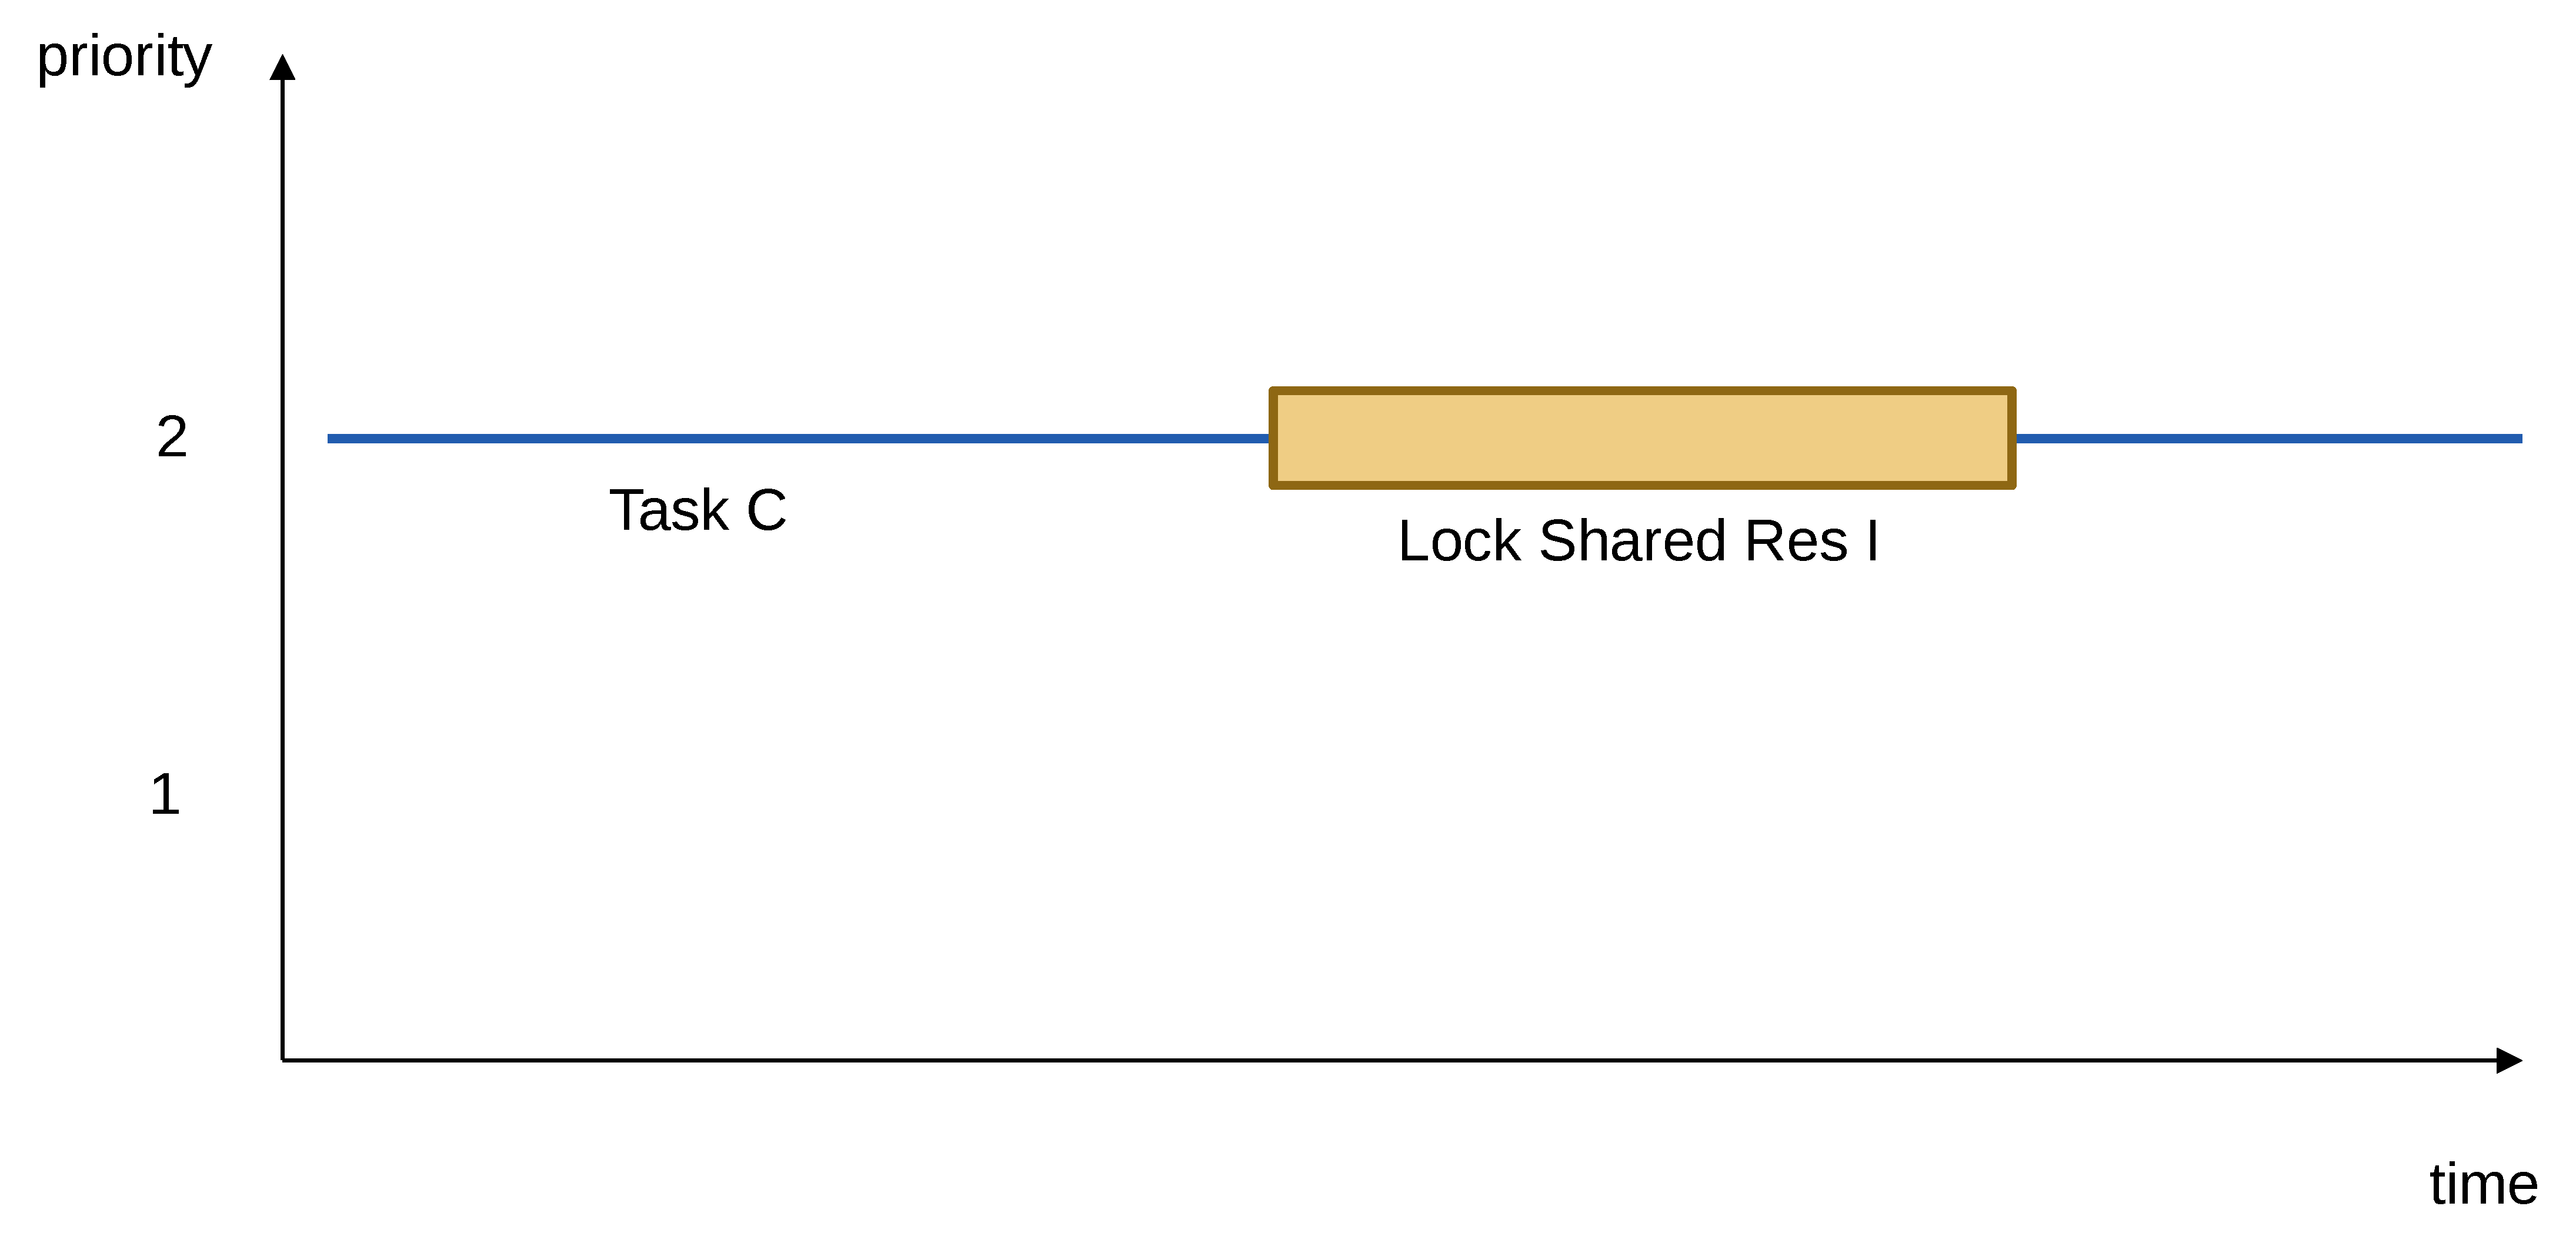
\includegraphics[width=\textwidth]{fig/locking_high_prio.svg.pdf}
  % Note: We do not have the SVG source file for the image above, so we have to put the PDF under version control.
  \caption{Locking of a Resource as highest Priority Task}%
  \label{fig:locking_high_prio}
  % Note: The `\label{}` can be on the line after the `\caption{}` if the `\caption{}` line ends with a comment.
\end{figure}

\begin{figure}
  \centerfloat
  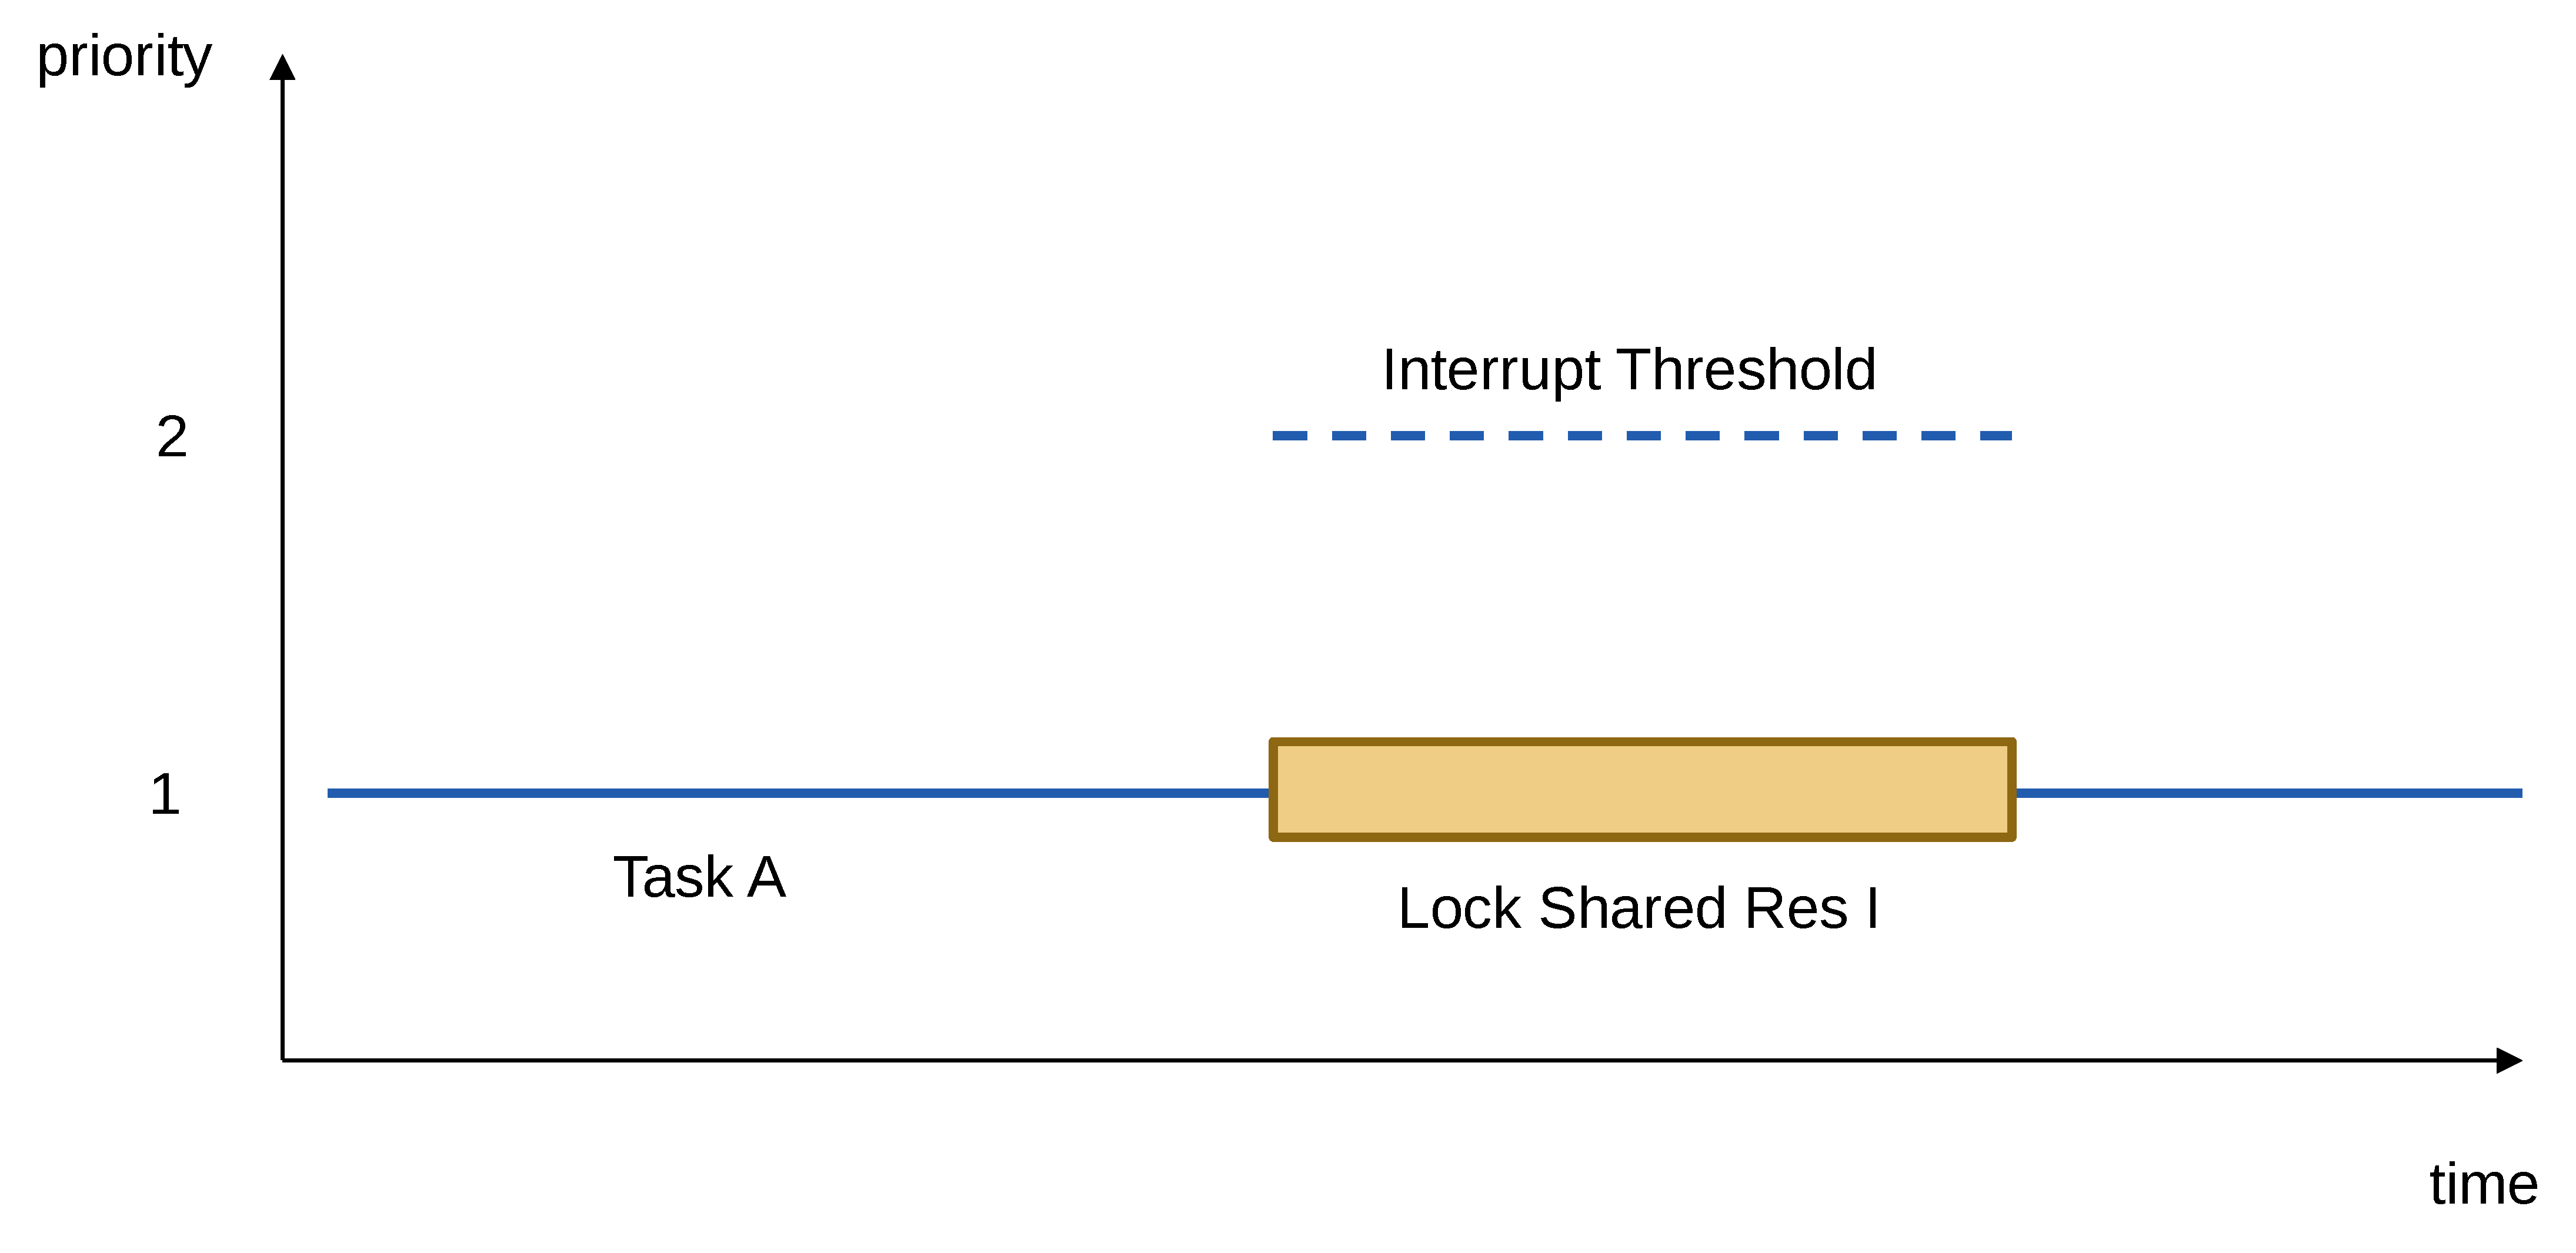
\includegraphics[width=\textwidth]{fig/locking_low_prio.svg.pdf}
  % Note: We do not have the SVG source file for the image above, so we have to put the PDF under version control.
  \caption{Locking of a Resource}%
  \label{fig:locking_low_prio}
  % Note: The `\label{}` can be on the line after the `\caption{}` if the `\caption{}` line ends with a comment.
\end{figure}

\section{Measurement Results}

In the following section, the results of the measurements that are described in section~\ref{sec:core_transitions} are presented.

Since locking of shared resources is already highly optimized by \gls{rtic}, it only uses between zero and four cycles, which is in the same range as the measurement uncertainties. Therefore, we do not show the locking measurements in the plots below, since they do not include any meaningful information.

\subsection{Original Implementation}

In the plot in figure~\ref{fig:plot_original}, 

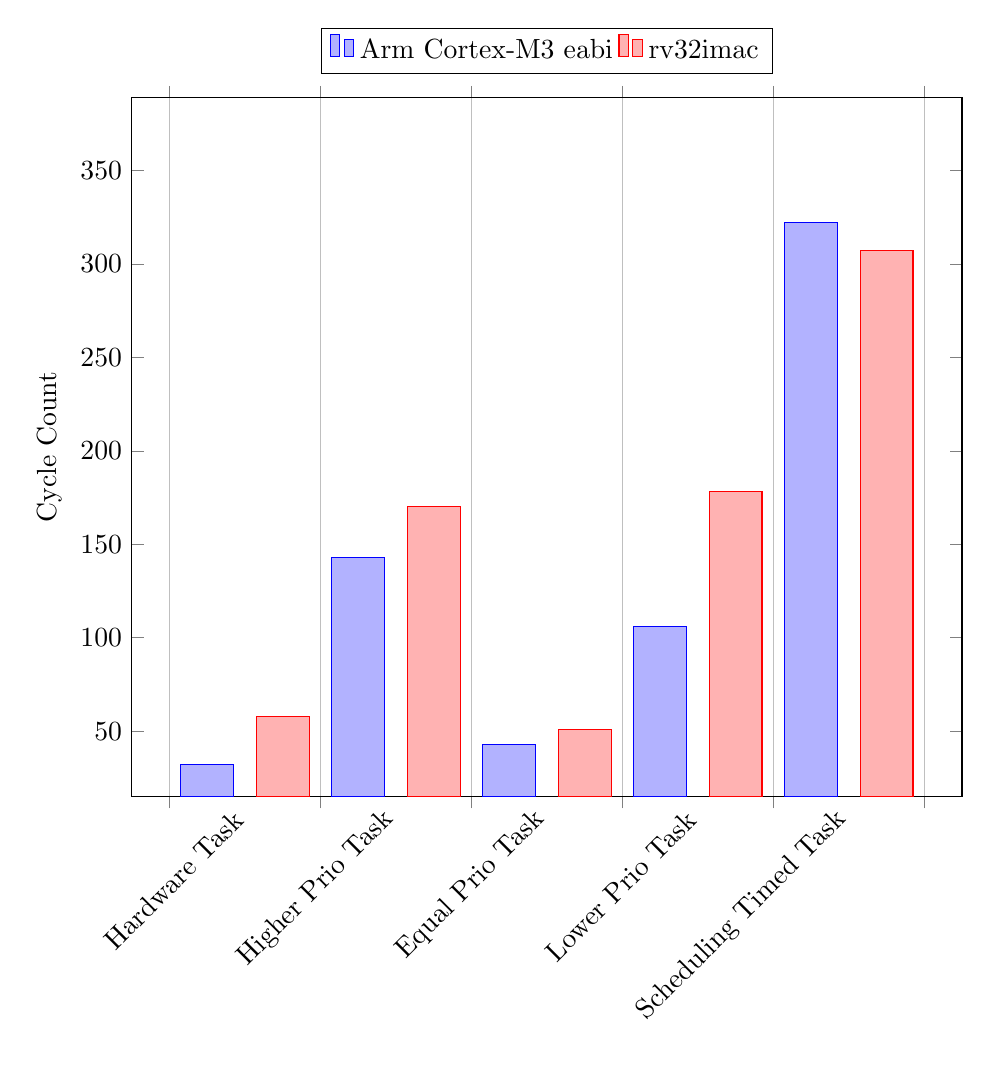
\begin{tikzpicture}
\label{fig:plot_original}
\begin{axis}[
	x tick label style={
		/pgf/number format/1000 sep=},
	ylabel=Cycle Count,
	enlargelimits=0.05,
	legend style={at={(0.5,1.1)},
	anchor=north,legend columns=-1},
	ybar interval=0.7,
        width=\textwidth,
        xticklabels={Hardware Task, Higher Prio Task, Equal Prio Task , Lower Prio Task, Scheduling Timed Task, Start Timed Task},
        xticklabel style={rotate=45, anchor=east}
]
\addplot 
	coordinates {(0,32) (1,143)
		 (2,43) (3,106) (4,322) (5,332)};
\addplot 
	coordinates {(0,58) (1,170)
		 (2,51) (3,178) (4,307) (5,372)};
\legend{Arm Cortex-M3 eabi,rv32imac}
\end{axis}
\end{tikzpicture}

\subsection{NXTI}

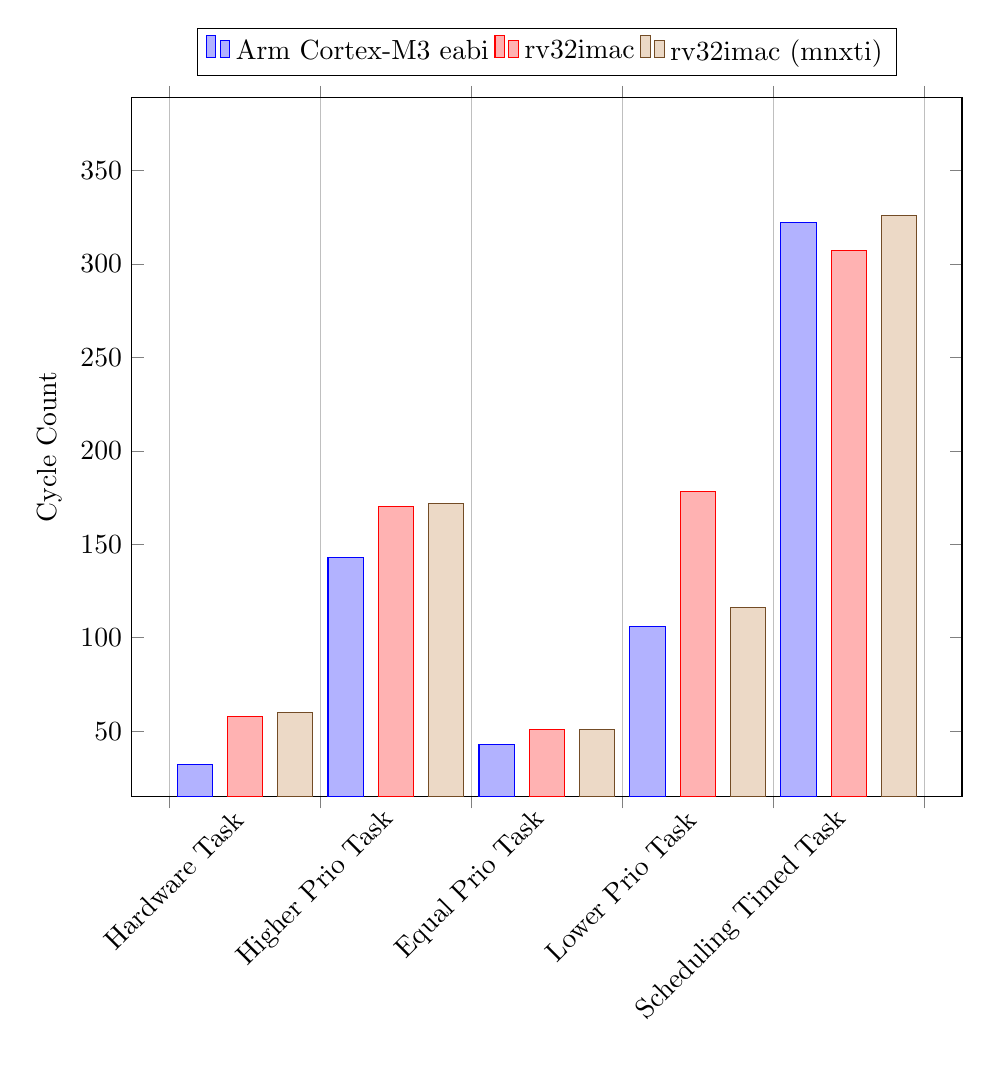
\begin{tikzpicture}
\label{fig:plot_nxti}
\begin{axis}[
	x tick label style={
		/pgf/number format/1000 sep=},
	ylabel=Cycle Count,
	enlargelimits=0.05,
	legend style={at={(0.5,1.1)},
	anchor=north,legend columns=-1},
	ybar interval=0.7,
        width=\textwidth,
        xticklabels={Hardware Task, Higher Prio Task, Equal Prio Task , Lower Prio Task, Scheduling Timed Task, Start Timed Task},
        xticklabel style={rotate=45, anchor=east}
]
\addplot 
	coordinates {(0,32) (1,143)
		 (2,43) (3,106) (4,322) (5,332)};
\addplot 
	coordinates {(0,58) (1,170)
		 (2,51) (3,178) (4,307) (5,372)};
\addplot 
	coordinates {(0,60) (1,172)
		 (2,51) (3,116) (4,326) (5,329)};
\legend{Arm Cortex-M3 eabi,rv32imac,rv32imac (mnxti)}
\end{axis}
\end{tikzpicture}

\subsection{E-Extension/EABI}

\pgfplotstableread[col sep=comma]{
Jahr, Facebook, Instagram, Snapchat, WhatsApp
0, 32,58,60,41
1,143,170,172,153
2,43,51,51,51
3,106,178,116,116
4,322,307,326,288
5,332,372,329,310
}\eextensiontable

\begin{tikzpicture}
\label{fig:plot_eextension}
\begin{axis}[
	x tick label style={
		/pgf/number format/1000 sep=},
	ylabel=Cycle Count,
	enlargelimits=0.05,
	legend style={at={(0.5,1.1)},
	anchor=north,legend columns=-1},
        ybar=0cm,
        xtick=data,
        %xmajorgrids=true,
        width=\textwidth,
        enlarge x limits={abs=0.8},
        xticklabels={Hardware Task, Higher Prio Task, Equal Prio Task , Lower Prio Task, Scheduling Timed Task, Start Timed Task},
        xticklabel style={rotate=45, anchor=east},
]
\addplot[draw=none,fill=ETHBlue]
	coordinates {(0,32) (1,143)
		 (2,43) (3,106) (4,322) (5,332)};
\addplot [draw=none,fill=ETHRed]
	coordinates {(0,58) (1,170)
		 (2,51) (3,178) (4,307) (5,372)};
\addplot  [draw=none,fill=ETHPurple]
	coordinates {(0,60) (1,172)
		 (2,51) (3,116) (4,326) (5,329)};
\addplot[ETHBlue,pattern=north east lines, pattern color=ETHBlue20]
	coordinates {(0,41) (1,153)
		 (2,51) (3,116) (4,288) (5,310)};
\legend{Arm Cortex-M3 eabi,rv32imac,rv32imac (mnxti),rv32imac (fastirq) estimation}
\end{axis}
\end{tikzpicture}
























In this chapter, you want to show that your implementation meets the objectives.
Start by briefly describing the type of results you have collected and how these results relate to the objectives.

\section{Evaluation setup}

Precisely describe your measurement/evaluation setup in a top-down manner.
For example:
\begin{itemize}
  \item If you used a development platform, which one and how was it configured?
  \item Which tools did you use?
  \item What input data set / program / signals / \ldots{} did you use?
    If your data set is very large, you should fully define and describe it in an appendix chapter and refer to that definition here using simple labels.
  \item If your implementation is configurable, which configuration(s) did you evaluate?
\end{itemize}

The information given here (with references to external work) should be sufficient to reproduce the setup you used for your measurements.

\section{Other sections}

Structure the rest of this chapter into sections.
For example, each section could discuss a different figure of merit or a different part of your implementation.
As usual, discuss structure and content in advance with your advisors.

\section{Comparison to related work}

Compare your results to those achieved by others working on similar problems.
This can be done in a separate section or directly in the sections above.

\section{Current limitations}

Demonstrating that your implementation meets the objectives is usually done by showing a lower bound on a given figure of merit.
Conversely, you should also illuminate the limitations of your implementation by showing upper bounds on these (or other appropriate) figures of merit.
Critically examining your ideas and their implementation trying to find their limits is also part of your work!



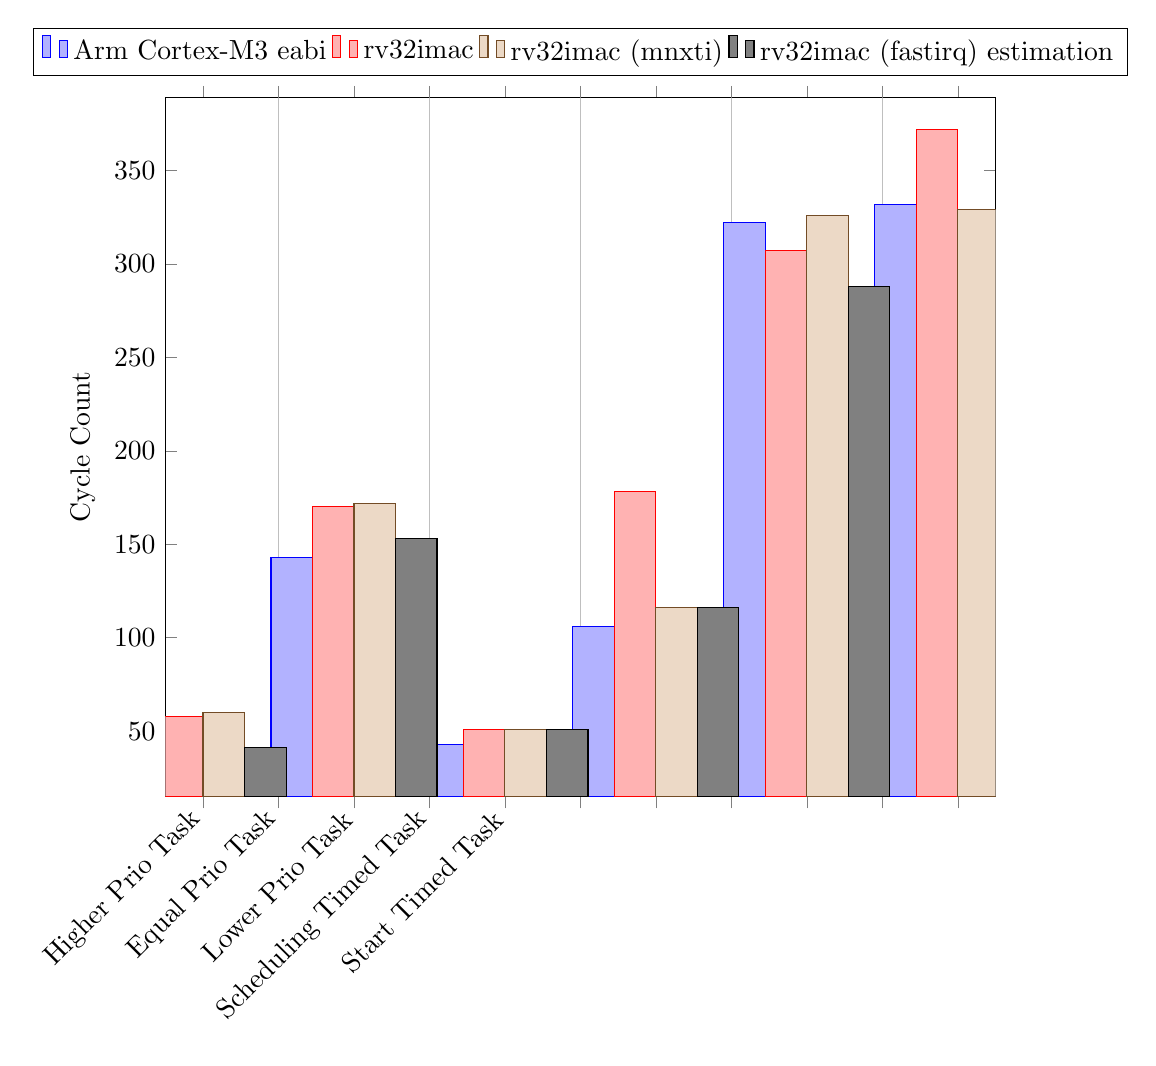
\begin{tikzpicture}
\begin{axis}[
	x tick label style={
		/pgf/number format/1000 sep=},
	ylabel=Cycle Count,
	enlargelimits=0.05,
	legend style={at={(0.5,1.1)},
	anchor=north,legend columns=-1},
	%ybar interval=1,
        ybar=0pt,
        bar width=15pt,
        width=\textwidth,
        xticklabels={Hardware Task, Higher Prio Task, Equal Prio Task , Lower Prio Task, Scheduling Timed Task, Start Timed Task},
        xticklabel style={rotate=45, anchor=east},
        extra x ticks={-0.5,0.5,1.5,2.5,3.5,4.5,5.5},
        extra x tick labels=\empty,
        extra x tick style={
            grid=major,
            % reset the tick length to the default value
            % (which otherwise would be the same as for the normal ticks
            %  which is set to zero in this case --> see above)
            xtick style={
                /pgfplots/major tick length=4pt,
            },
        },
]
\addplot 
	coordinates {(0,32) (1,143)
		 (2,43) (3,106) (4,322) (5,332)};
\addplot 
	coordinates {(0,58) (1,170)
		 (2,51) (3,178) (4,307) (5,372)};
\addplot 
	coordinates {(0,60) (1,172)
		 (2,51) (3,116) (4,326) (5,329)};
\addplot 
	coordinates {(0,41) (1,153)
		 (2,51) (3,116) (4,288) (5,310)};
\legend{Arm Cortex-M3 eabi,rv32imac,rv32imac (mnxti),rv32imac (fastirq) estimation}
\end{axis}
\end{tikzpicture}